\documentclass[aip, jcp, reprint, onecolumn]{revtex4-2}

\bibliographystyle{apsrev4-2}

\usepackage{physics}
\usepackage{amsmath}
\usepackage{amssymb}
\usepackage{mathtools}
\usepackage{graphicx}
\usepackage{dcolumn}
\usepackage[colorlinks=true, linkcolor=black, urlcolor=blue, citecolor=black, anchorcolor=black]{hyperref}

\graphicspath{{"figures/"}}
\begin{document}
%Title of paper
\title{Coherent Hyper-Raman Four Wave Mixing Vibrational Spectroscopy}


\author{Ryan P. McDonnell} 
\author{Daniel D. Kohler}
\author{John C. Wright} \email{wright@chem.wisc.edu}

\affiliation{Department of Chemistry, 
        University of Wisconsin - Madison, 
        Madison, Wisconsin 53706, 
        United States of America}

\date{\today}

\begin{abstract}
Nonlinear, four wave mixing vibrational spectroscopies are often used to probe intramolecular vibrational coupling and relaxation dynamics in isotropic media.
Three wave mixing vibrational spectroscopies, such as vibrational sum frequency generation (vSFG) are similarly used to probe the spectroscopy and dynamics of interfacial species.
Most of these methods rely on infrared and/or Raman transitions to generate output. 
Implementing a nonlinear spectroscopy involving hyper-Raman transitions, first appearing at third order perturbation theory, can provide a useful analogue to infrared and Raman based nonlinear spectroscopies to understand the spectroscopy and dynamics of isotropic systems.
Hyper Difference Frequency Generation (Hyper-DFG, or HDFG) spectroscopy, also known as singly vibrationally enhanced spectroscopy (SIVE), is an underdeveloped, hyper-Raman based four wave mixing vibrational spectroscopy. 
Despite several experimental reports on HDFG, its spectroscopic properties have not been fully explored.
To this end, we explore the selection rules and response functions of HDFG spectroscopy.
Through the hyper-Raman $A,B$ terms, we explore the selection rules of singly and doubly resonant HDFG spectroscopy, and show HDFG is a hybrid IR-hyper-Raman technique.
Since all infrared active modes have non-zero hyper-Raman activity, this makes HDFG a type of upconverted infrared spectroscopy.
HDFG is found to be uniquely sensitive to non-Condon effects in centrosymmetric species.
Through a simple comparison test, HDFG output is shown to be similar in magnitude to vibrational sum frequency generation (vSFG).
Since HDFG can also be implemented as a two beam experiment, similar to vSFG, this makes HDFG a spectroscopy feasible for practitioners of vSFG.
Through a simple treatment of orientational averaging, HDFG provides a simple method to extract hyper-Raman hyperpolarizabilities ($\beta$) of infrared active vibrations.
HDFG shows promise as a method to disentangle vibrational spectra and dynamics in isotropic systems without need for anharmonicities.

\end{abstract}

\maketitle

\section{Introduction}
Coherent multidimensional spectroscopy (CMDS) is a family of three and four wave mixing methods which form the optical analogue of multidimensional nuclear magnetic resonance (NMR) spectroscopy.\cite{Cho2008}
Multiresonant, four wave mixing CMDS experiments, first proposed by Oudar and Shen in 1980,\cite{RN307} directly probe coupling and correlations between different vibrational, electronic, and vibronic states. \cite{RN281, RN103, Cho2008} 
Four wave mixing CMDS has resolved anharmonicities, ultrafast dynamics, and other intramolecular couplings in numerous systems. \cite{Cho2008, Gaynor2017, Ziegler2018, Ogilvie2019, Bonn2021, RN325}

Not all CMDS methods are used to dissect intramolecular couplings.\cite{Shen1987_CPL}
The most well known example of such a spectroscopy is vibrational sum frequency generation (vSFG), a three wave mixing technique used to probe vibrational structure and dynamics at interfaces. \cite{Shen1987_CPL, RN224}
Non-parametric, hyper difference frequency generation (hyper-DFG, or HDFG) spectroscopy, similar to difference frequency generation (\autoref{fig:comparisonwmel}), is a four wave mixing method which, when detuned from  electronic resonances, does not probe intramolecular couplings. 
HDFG was one of the first infrared CMDS methods to successfully discriminate against non-resonant background.\cite{RN351, RN352}
HDFG has also been referred to as singly vibrationally enhanced (SIVE) spectroscopy. \cite{RN352}
In HDFG, an infrared pulse is resonant with a vibrational mode, and two other input pulses are used to stimulate a scattering process.
HDFG was documented long ago to have characteristics similar to both infrared spectroscopy and spontaneous hyper-Raman scattering. \cite{RN352}
Hyper-Raman scattering is the two photon analogue to Raman scattering. \cite{Terhune1965, Cyvin1965, Andrews1978}
Hyper-Raman scattering cross sections are commonly several orders of magnitude smaller than Raman scattering cross sections, making hyper-Raman a difficult process to detect.\cite{RN515, Kelley2010} 
However, unlike Raman spectroscopy, all infrared active modes are hyper-Raman active, which allows infrared active modes to be probed through an inelastic scattering event. \cite{Andrews1978}
The different selection rules of hyper-Raman scattering make it a unique alternative to Raman scattering to understand vibrational spectra, electronic structure and vibronic coupling in molecular systems. \cite{Olson2018}
Several authors have proposed parametric six wave mixing techniques as the coherent analogue of hyper-Raman scattering. \cite{Berger1978, Cho1997, Cho1998}
However, since most six wave mixing methods cascade into four wave mixing processes and their homodyned output would be dependent upon the hyper-Raman scattering cross section, \cite{RN243,Cho1997, Cho1998, Cho2000_Cascade} it is preferable to investigate four wave mixing analogues to hyper-Raman scattering.

\begin{figure*}[!htbp]
	\centering
	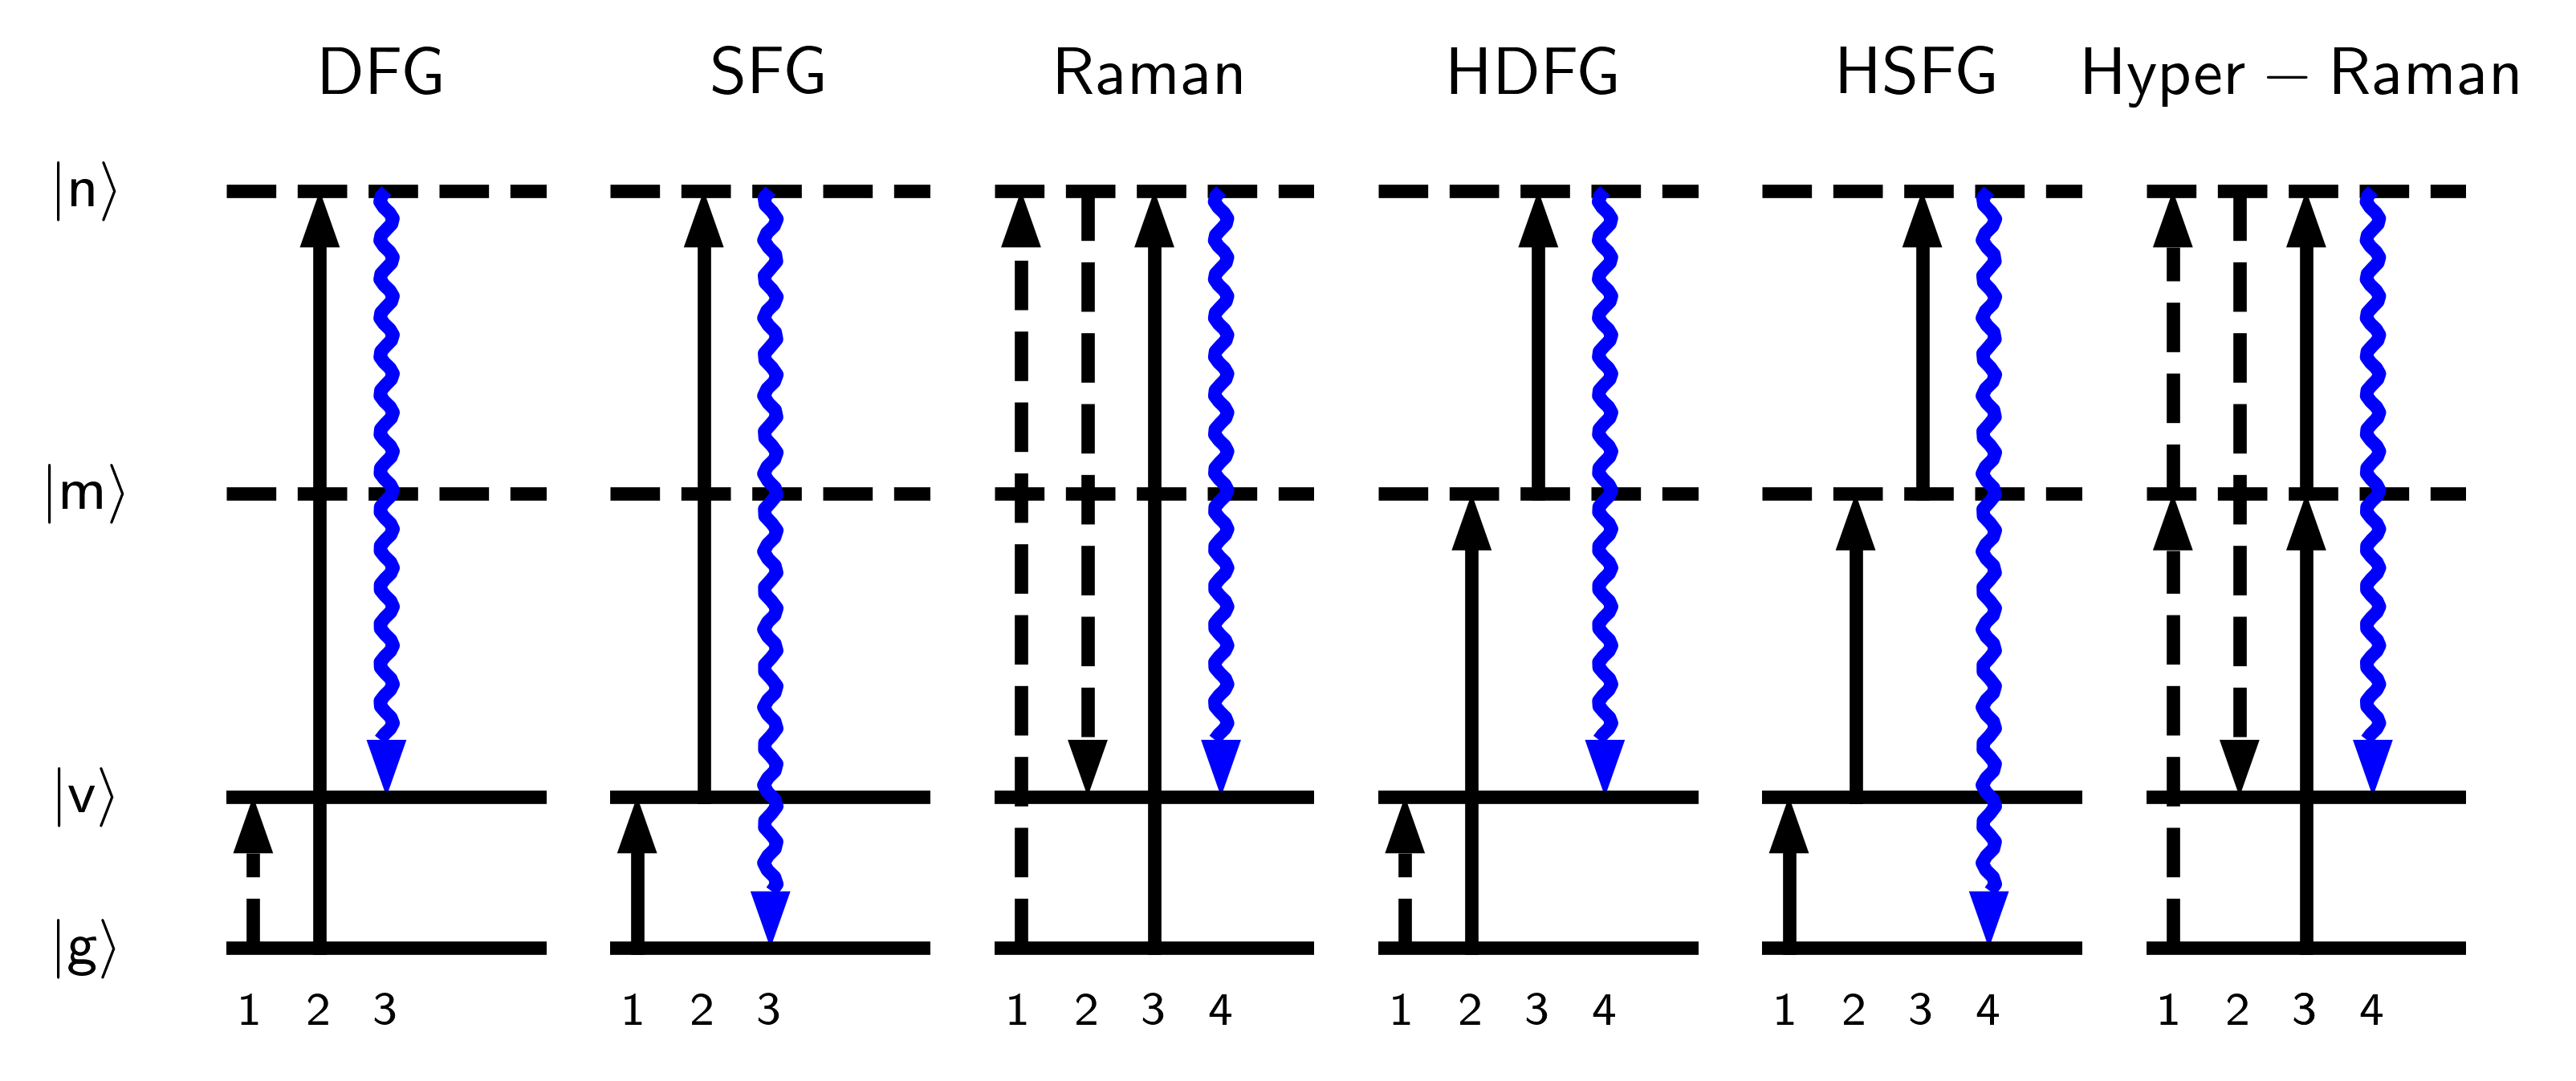
\includegraphics[width=6.66in]{comparisonwmel.png}
	\caption{Wave Mixing Energy Level (WMEL) diagrams of difference frequency generation (DFG), sum frequency generation (SFG), spontaneous Raman scattering, hyper difference frequency generation (HDFG), hyper sum frequency generation (HSFG) and spontaneous hyper-Raman scattering relevant to this discussion. \cite{RN286}
	Solid and dashed horizontal lines indicate real and virtual states, whereas solid and dotted arrows indicate ket and bra side transitions, respectively. 
	}
	\label{fig:comparisonwmel}
\end{figure*}

While HDFG showed promise as an upconverted infrared spectroscopy method, it was quickly supplemented by a doubly vibrationally resonant method, doubly vibrationally enhanced (DOVE) spectroscopy, to investigate intra- and intermolecular vibrational coupling. \cite{RN345, RN101, Cho2000}
As a result, investigations of HDFG stagnated; to date, there are roughly a dozen studies which report on HDFG. \cite{Zilian1994, RN350, RN416, RN351, RN352, RN353, Chen1998, RN362, RN418, Bonn2024, McDonnell2024}
Recent reports highlight non-negligible HDFG interference in DOVE experiments as well as the suitability of HDFG pathways to interpret ultrafast relaxation dynamics in isotropic systems. \cite{Bonn2024, McDonnell2024}
These reports motivate deeper analysis of HDFG spectroscopy. 

Fully coherent, ultrafast probes of vibronic coupling would yield insight into processes that control ultrafast electronic relaxation in molecular and biological systems. \cite{Bredenbeck2015, Arsenault2021}
Some years ago, Cho proposed a parametric, doubly resonant infrared/visible pathway to probe vibronic coupling in isotropic systems. \cite{Cho2001}
In this method, a single infrared pulse is resonant with a vibrational mode, and a two photon absorption event from a near infrared (NIR) or visible pulse resonant with an electronic or vibronic state is used to generate the four wave mixing signal.
The non-parametric pathways similar to this method are referred to herein as doubly resonant HDFG (DR-HDFG).
Methods analogous to DR-HDFG, where two photon absorption from the infrared pulse and one photon absorption from the visible pulse is used to generate output, i.e., stimulated Raman processes, have been reported. \cite{RN301, RN120} 

An experimental complexity in executing Raman based four wave mixing experiments is the demand of three separate input pulses, often at different frequencies.
For example, in the case of DOVE, two of the three inputs must be tunable infrared pulses. \cite{RN345} 
Only recently have methods been developed for seamless tuning and scanning of ultrafast optical parametric amplifiers across swaths of frequency space. \cite{RN162, McDonnell2024}
Since HDFG demands only a single resonance to be scanned, the experiment can be performed using two input pulses: one tunable, infrared OPA to scan across vibrational resonances, and a two photon absorption from the signal process of a separate OPA, or output from the oscillator which pumps the infrared OPA. \cite{Wang2021}
As such, laboratories experienced in sum frequency generation (SFG) spectroscopy can perform HDFG spectroscopy to understand bulk dynamics and spectroscopy using nearly the same setup.

Inspired by recent work which demonstrated the presence of HDFG in ultrafast DOVE and terahertz-IR-visible (TIRV) experiments, we investigate the parameters which result in both SR and DR-SIVE output. \cite{Cho2000, Bonn2024, McDonnell2024}
This paper is organized as follows.
In \autoref{steadystate}, we identify the selection rules that drive singly and doubly resonant HDFG, first through the Placzek approximation, and then through hyper-Raman $A,B,C$ coefficients.
After developing selection rules, some quantitative aspects of HDFG, particularly a comparison of vSFG and HDFG output and a method to extract hyper-Raman hyperpolarizabilities ($\beta_{ijk}$) from HDFG spectra, are discussed in \autoref{quant}.
Finally, mixed time-frequency domain HDFG is discussed in \autoref{mixeddomain}. 

\section{Steady State HDFG Spectroscopy}\label{steadystate}

Singly resonant hyper difference generation spectroscopy (HDFG) spectroscopy has potential to provide deeper insight into single quantum decoherence times and molecular orientation in condensed systems.
Similarities between HDFG spectroscopy, infrared spectroscopy and spontaneous hyper-Raman scattering have been noted previously. \cite{RN352, Bonn2024, McDonnell2024}
In this section, we investigate the steady state properties of HDFG and make the connections between HDFG and hyper-Raman scattering explicit.

It is useful to expose relationships between transition dipoles, Raman polarizabilities and hyper-Raman hyperpolarizabilities in the driven limit. \cite{Simpson2004}
In the driven limit, under the electric dipole approximation, the I$^{th}$ component of the third order nonlinear output polarization, ${P}^{(3)}_I$, of any four wave mixing process, induced by electric fields E, at output frequency $\omega_4$ is written as (using Einstein summation) \cite{RN307}
\begin{equation} \label{polarization}
{P}^{(3)}_I (\omega_4)  = \chi^{(3)}_{IJKL} E_J E_K E_L 
\end{equation}
where $\chi^{(3)}_{IJKL}$ is the IJKL element of the third order electrical susceptibility, a rank four tensor, generally written as
\begin{equation}
	\chi^{(3)}_{IJKL} = NF(\omega_4) \langle \gamma_{ijkl} \rangle
\end{equation}
where N is a number density, F is the Lorentz local field factor, and $\gamma_{ijkl}$ is the third order polarizability (i.e., second hyperpolarizability). 
The brackets indicate an orientational average. 
Uppercase letters refer to laboratory frame coordinates and lower case letters refer to molecular frame coordinates.

To make the connection between HDFG and hyper-Raman scattering, we investigate its gross selection rules.
By propagating density matrix elements in the steady state limit under the rotating wave approximation, the HDFG hyperpolarizability is \cite{RN133}
\begin{equation}\label{sivegamma}
		\gamma_{ijkl}^{vg} =	- \sum_{m, n} \frac{1}{\varepsilon_0} \frac{1}{4D} \frac{1}{\hbar^3} \frac{\mu^{vn}_{i} \mu^{nm}_{j} \mu^{mg}_{k} \mu^{gv}_{l} }{\Delta_{nv} \Delta_{mv}\Delta_{gv}}  \rho_{gg}
\end{equation}
where: $\mu^{ab}_{j}$ is the $j^{th}$ element of $\mel{a}{\vec{\mu}}{b}$, $\Delta_{kl} = \omega_{kl} - \omega_{j} - i\Gamma_{kl}$ (also known as a resonance denominator), $\omega_j$ is the frequency of the j$^{th}$ input field, $\Gamma_{kl}$ is the dephasing of $\rho_{kl}$ and $\rho_{gg}$ is the ground state population.
D, the Maker-Terhune degeneracy factor, accounts for permutation symmetry in $\gamma_{ijkl}$.\cite{RN134} 
For a HDFG experiment using two (three) distinct input fields, D = 3 (6).

\subsection{Placzek Method}
We first investigate the HDFG selection rules through a Placzek type formalism.
Contracting over the virtual states forms the hyper-Raman hyperpolarizability $\beta$.\cite{Long1970} 
Assuming $\omega_2$, $\omega_3$ are significantly detuned from any resonance (\autoref{fig:comparisonwmel}),\cite{Placzek1934, Long1970, Altmann1982} \autoref{sivegamma} is written as 
\begin{equation}\label{sivebeta}
	\gamma_{ijkl}^{vg} =	-\frac{1}{\varepsilon_0} \frac{1}{4D \hbar}\frac{\beta^{vg}_{ijk} \mu^{gv}_{l}}{\Delta_{gv}} \rho_{gg}
\end{equation}
All infrared active transitions are hyper-Raman active, making HDFG allowed for any infrared active transition. \cite{Andrews1978}
It is important to note that the symmetry properties of $\beta_{ijk}$ change dependent upon whether $\omega_2$ and $\omega_3$ are degenerate. \cite{Denisov1986, Kozich2007}
Taylor expanding the dipole and first hyperpolarizability operators in terms of an n$^{\text{th}}$ reduced normal mode coordinate $Q_n$ to $\order{Q_n}$ about equilibrium as\cite{Long1970, Shen90}
\begin{subequations}
	\begin{equation}
		\mu_l = \mu_{l,0} + \left(\frac{\partial \mu_l}{\partial Q_n}\right)_0 Q_n 
	\end{equation}
	\begin{equation}
		\beta_{ijk} = \beta_{ijk,0} + \left(\frac{\partial \beta_{ijk}}{\partial Q_n}\right)_0 Q_n
	\end{equation}
\end{subequations}
and substituting into \autoref{sivebeta} gives the HDFG hyperpolarizability to $\order{Q_n}$ as \begin{equation}\label{SIVEselection}
	\gamma_{ijkl}^{vg} =	-\frac{1}{\varepsilon_0} \frac{1}{8D m_n \omega_{vg}}  \frac{1}{{\Delta_{gv}}} \ \left(\frac{\partial \beta^{vg}_{ijk}}{\partial Q_n}\right)_0 \left({\frac{\partial \mu^{gv}_{l}}{\partial Q_n}}\right)_0  \rho_{gg}
\end{equation}
where $\mel{v}{Q_n}{g} = \sqrt{\frac{\hbar}{2\omega_{vg}}}$ if $v-g = \pm 1$.  \cite{RN230}
Since this expression is non-zero in the harmonic oscillator limit, HDFG output is allowed for harmonic transitions. 
Similar to SFG, HDFG does not demand anharmonic ground state potential energy surfaces for spectral output. \cite{Shen94, Cho2000}
This selection rule is generally valid for any HDFG or hyper sum frequency generation (HSFG) process in the $-\vec{k}_1 + \vec{k}_2  + \vec{k}_3$ and $\vec{k}_1 + \vec{k}_2  + \vec{k}_3$ phasematching geometries when $\omega_2$ and $\omega_3$ are sufficiently detuned from any resonance.

\begin{figure}[!htbp]
	\centering
	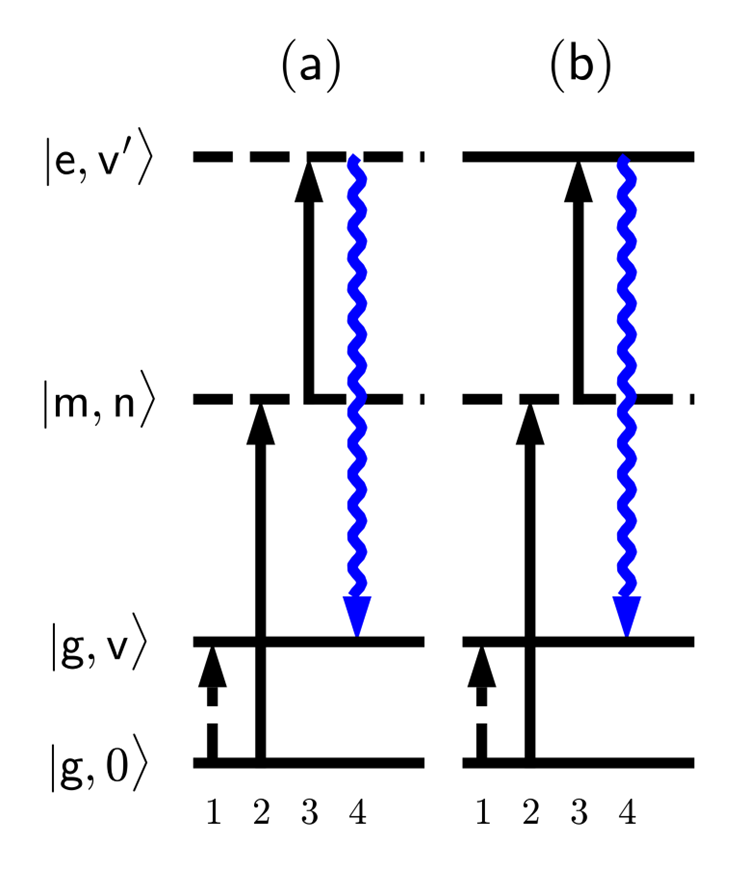
\includegraphics[width=3.375in]{hdfg.png}
	\caption{WMEL diagrams of (a) singly resonant and (b) doubly resonant HDFG. 
	}
	\label{fig:hdfg}
\end{figure}
\subsection{Albrecht Type Expansion}
While Placzek type arguments provide the general source of HDFG output, it is insightful to interpret the origin of signal in terms of $A,B,C$ terms, analogous to those found in Albrecht's treatment of Raman spectroscopy.\cite{Albrecht1961, Ziegler1988} 
We write $\beta_{ijk}$ in \autoref{SIVEselection} using the hyper-Raman ABC formalism introduced by Chung and Ziegler to understand how vibronic coupling manipulates selection rules for singly and doubly resonant HDFG (\autoref{fig:hdfg}). \cite{Ziegler1988}
To employ this formalism, we write the states in terms of a Born-Oppenheimer basis $\ket{a,b}$, where $\ket{a,b} = |a(Q)) \otimes \ket{b}$ for electronic states $\{|a(Q))\}$ and vibrational states $\{\ket{b}\}$ (i.e., adiabatic approximation). \cite{BornOppenheimer, Tang1970}
The dependence of the electronic states on the adiabatic parameter $Q$ is suppressed for simplicity.
The states are labeled as shown in \autoref{fig:hdfg}.
For consistency with previous reports, we use $\vec{R}$ to denote electric transition dipole moments; $\vec{\mu}$ is reserved for transitions on the ground electronic state. \cite{Tang1970}
Following the approach which gave \autoref{sivegamma}, we find
\begin{equation}\label{drgamma_notaylor}
	\gamma_{ijkl} = -\frac{1}{\varepsilon_0} \frac{1}{4D \hbar^3} \sum_{m,n,e,v'} \frac{
		R_{i}^{gv, ev'} 
		R_{j}^{ev',mn} 
		R_{k}^{mn,g0} 
		R_{l}^{g0,gv} 
	}{\Delta_{g0,gv}
		\Delta_{ev', mn}
		\Delta_{mn, g0}
	}
\end{equation}
where $R_{i}^{ab,cd}$ is the i$^{th}$ element of $\mel{a,b}{\vec{R}}{c,d}$.
It is common in the hyper-Raman community to write $\Delta_{ev', mn} \Delta_{mn, g0} = \Delta_{ev', g0}$.
Using our definition of vibronic states, we write $\vec{M}^{ab} = (a|\vec{M}|b)$ so that, for example,
$R_{i}^{gv,ev'} = \mel{v}{M_i^{ge}}{v'}$.
Chung and Ziegler showed some years ago that expanding $\vec{M}^{ij}$ to $\order{Q}$ \textit{about the equilibrium point of the ground state potential surface} as
$\vec{M}^{ij} = \vec{M}^{ij}_0 + \sum_z \frac{\partial\vec{M}^{ij}}{\partial Q_z} Q_z$
yields $A, B, C$ coefficients similar to those in the Albrecht formalism of Raman scattering, \cite{Albrecht1961, Ziegler1988} so that
\begin{equation}
		\gamma_{ijkl} \sim \frac{(A_{ijk} + B_{ijk} + C_{ijk})\mel{v}{\mu_{l}}{0}} {\Delta_{g0,gv}}
\end{equation}
The $A$ term depends upon $\order{Q^0}$ transitions (i.e., Condon approximation), the $B$ term depends upon $\order{Q}$ transitions, and the $C$ term depends on $\order{Q^2}$ transitions. 
The C term is suppressed in the following discussion as it depends on one and two photon forbidden transitions. \cite{Ziegler1988, Neddersen1989, Bonang1992}
Note that some reports obtain $A, B$ coefficients through a Herzberg-Teller expansion of the electronic states to expose vibronic couplings in terms of $\partial H / \partial Q$, where H is the electronic Hamiltonian.\cite{HerzbergTeller1933, Petrov1985, Neddersen1989, Baranov1990}
This approach is not used here as the expansion of $\vec{M}^{ij}$ in normal mode coordinates provides sufficient physical insight into hyper-Raman selection rules. 

By contracting over the virtual vibrational states $\ket{n}$, the $A$ and $B$ coefficients, where $B = B_1 + B_2$, are written as
\begin{widetext}
\begin{subequations}\label{ABterms}
\begin{equation}
	\begin{split}
		A_{ijk} = \frac{1}{\hbar^2}\sum_{m,e,v'} M^{ge}_{0,i} 
		M^{em}_{0,j} 
		M^{mg}_{0,k}
		 \langle v | v' \rangle
		 \langle v' | 0 \rangle 
		 \frac{1}{\Delta_{ev', g0}}
		 \\
	\end{split}
\end{equation}
	\begin{equation}
		\begin{split}
			B_{1_{ijk}} &= \frac{1}{\hbar^2} \sum_{m,e,v',z} M^{ge}_{0,i} \langle v | v' \rangle \left(
			 \frac{\partial M^{em}_{j}}{\partial Q_z} M^{mg}_{0,k} \mel{v'}{Q_z}{0} 
			+M^{em}_{0,j} \frac{\partial M^{mg}_{k}}{\partial Q_z} \mel{v'}{Q_z}{0} \right) \frac{1}{\Delta_{ev', g0}}\\
		\end{split}
	\end{equation}
	\begin{equation}
	\begin{split}
			B_{2_{ijk}} = \frac{1}{\hbar^2} \sum_{m,e,v',z} \frac{\partial M^{ge}_{i}}{\partial Q_z} M^{em}_{0,j} 
			M^{mg}_{0,k} \mel{v}{Q_z}{v'} 
			\langle v' | 0 \rangle 
			\frac{1}{\Delta_{ev', g0}}
	\end{split}
	\end{equation}
\end{subequations}
\end{widetext}
where terms such as $\langle a | b \rangle$ and $\mel{a}{Q}{b}$ are Franck-Condon factors and Herzberg-Teller-type integrals, respectively. 
These expressions are valid for both singly and doubly resonant HDFG, but based upon the resonance schemes, further simplifications can be made (\textit{vide infra}).
\subsubsection{Singly Resonant HDFG}
In the case of singly resonant HDFG, $\omega_3$ is also detuned from any resonance, which permits contraction over ${v'}$ as the dependence on $\ket{v'}$ in the resonance denominator can be neglected. 
This limit is usually reached when $\abs{\omega_{ev',g0} - (\omega_2 + \omega_3)} \gg 2\Gamma_{ev',g0}$.
In such a limit, assuming a normal mode basis, we see for singly resonant HDFG that 
\begin{subequations}
\begin{equation}
	A_{ijk} \sim \sum_{v'}\langle v | v' \rangle \langle v' | 0 \rangle = \delta_{v0} = 0
\end{equation}
\begin{equation}
	B_{1_{ijk}} = \frac{1}{\hbar^2} \sum_{m,e,z} M^{ge}_{0,i} \left( 
	\frac{\partial M^{em}_{j}}{\partial Q_z} M^{mg}_{0,k}
	+M^{em}_{0,j} \frac{\partial M^{mg}_{k}}{\partial Q_z} \right) \frac{\mel{v}{Q_z}{0}}{\Delta_{e, g0}}
\end{equation}
\begin{equation}
	B_{2_{ijk}} = \frac{1}{\hbar^2} \sum_{m,e,z} \frac{\partial M^{ge}_{i}}{\partial Q_z} M^{em}_{0,j} 
	M^{mg}_{0,k}  
	\frac{\mel{v}{Q_z}{0}}{\Delta_{e, g0}}
\end{equation}
\end{subequations}
i.e., A$_{ijk}$ vanishes, but B$_{ijk}$ is non-zero, for singly resonant HDFG. 
When $\abs{\omega_{ev',g0} - (\omega_2 + \omega_3)} \gtrsim \Gamma_{ev',g0}$, $\Re(\frac{1}{\Delta_{ev', g0}})$ can allow for small $A$ term contributions (cf. the long tail associated with the $A$ term of DR-HDFG as presented in \autoref{fig:doubres_spec}b).
As such, $A$ usually only vanishes when $\omega_2, \omega_3$ are highly detuned from electronic states. 
In the limit where $A$ vanishes, the singly resonant HDFG susceptibility can be approximated as $\chi^{(3)}_{IJKL} \sim \langle B_{ijk} \mu_l \rangle$, or, while a vibrational mode must be infrared active for HDFG output, vibronic activity is necessary for singly resonant HDFG response.
The breakdown of the Condon approximation in singly resonant HDFG supports the relatively small HDFG $\chi^{(3)}$ values ($\sim$ order of magnitude larger than nonresonant background) for hexane and similar organic solvents. \cite{RN350, RN351, RN353}

\subsubsection{Doubly Resonant HDFG}
The selection rules for DR-HDFG are different. 
DR-HDFG (where a vibrational and vibronic state are resonantly coupled) can provide a tool for measuring vibronic coupling, analogous to fully resonant DFG. \cite{Dick83_1, Shen94}
Many multi-resonant nonlinear spectroscopies have been developed to resolve vibronic coupling in molecular samples. \cite{Carlson1990, Gaynor2017, RN276}
DR-HDFG provides methods to investigate vibronic coupling with only two laser pulses.
Experimentally, DR-HDFG would provide identical information to DR-HSFG, but only DR-HDFG is phasematchable in media with normal indices of refraction, so we focus our attention on DR-HDFG. \cite{RN278}
DR-HDFG output is dependent upon the $A,B$ terms prior to contraction over $\ket{v'}$ as written in \autoref{ABterms}. 

Unlike a spontaneous hyper-Raman experiment, a DR-HDFG experiment selectively excites quanta in ground state vibrational modes (\autoref{fig:hdfg}), making it similar to a stimulated hyper-Raman experiment. 
As a result, the spectrum along the electronic scanning axis ($\omega_2 + \omega_3$) is significantly simplified as the coupling between the vibronic states are isolated to only $\ket{g,0}$ and $\ket{g,1}$, assuming the infrared pulse puts a single quantum in the normal mode of interest ($\ket{g,1}$).
By working only in terms of a single normal mode (i.e. removing the sum over $z$) and assuming electronic transitions occur only between $|g), |e)$ and that $v =1$, $v' = \{0,1,2\}$, the A and B terms are rewritten as 
	\begin{subequations}\label{ABterms_DR}
		\begin{equation}
			\begin{split}
				A_{ijk} = \frac{1}{\hbar}\sum_{v'} M^{ge}_{0,i} 
				\Lambda^{eg}_{0,jk}
				\langle 1 | v' \rangle
				\langle v' | 0 \rangle 
				\frac{1}{\Delta_{ev',g0}}
				\\
			\end{split}
		\end{equation}
		\begin{equation}
			\begin{split}
				B_{1_{ijk}} &= \frac{1}{\hbar} \sum_{v'} M^{ge}_{0,i} \langle 1 | v' \rangle 
				\frac{\partial \Lambda^{eg}_{jk}}{\partial Q} \mel{v'}{Q}{0} 
				\frac{1}{\Delta_{ev', g0}}\\
			\end{split}
		\end{equation}
		\begin{equation}
			\begin{split}
				B_{2_{ijk}} = \frac{1}{\hbar} \sum_{v'} \frac{\partial M^{ge}_{i}}{\partial Q} 
				\Lambda^{eg}_{0,jk} 
				\mel{1}{Q}{v'} 
				\langle v' | 0 \rangle 
				\frac{1}{\Delta_{ev',g0}}
			\end{split}
		\end{equation}
	\end{subequations}
where the electronic two photon absorption operator, $\Lambda$ was invoked to simplify summation over virtual states. \cite{McClain1977}
The constraint of $v' = \{0,1,2\}$ is done for simplicity. 

The selection rules for DR-HDFG follow more clearly from \autoref{ABterms_DR}.
It is clear from \autoref{ABterms_DR} that the Condon approximation breaks down for centrosymmetric molecules, as inversion centers invoke strict parity constraints that make states not accessible via both one and two photon transitions. \cite{Milojevich2013, RN230}
This makes DR-HDFG a unique tool for studying the electronic structure of centrosymmetric species in isotropic media, as it is sensitive to non-Condon effects. \cite{Olson2018}
The $B_1$ and $B_2$ terms involve different types of vibronic coupling pathways.
In $B_1$, the Herzberg-Teller coupling is associated with the two-photon absorption process, whereas in $B_2$, the Herzberg-Teller coupling is associated with one-photon emission.
As such, $B_1$ contributions to a DR-HDFG spectrum will be sensitive to vibronic coupling between the ground state of a mode and vibrational states on the $|e)$ surface. 
$B_2$ contributions are sensitive to vibronic coupling between the first excited state of a mode $\ket{g,1}$ and vibrational states on $|e)$.

\begin{figure*}[!htbp]
	\centering
	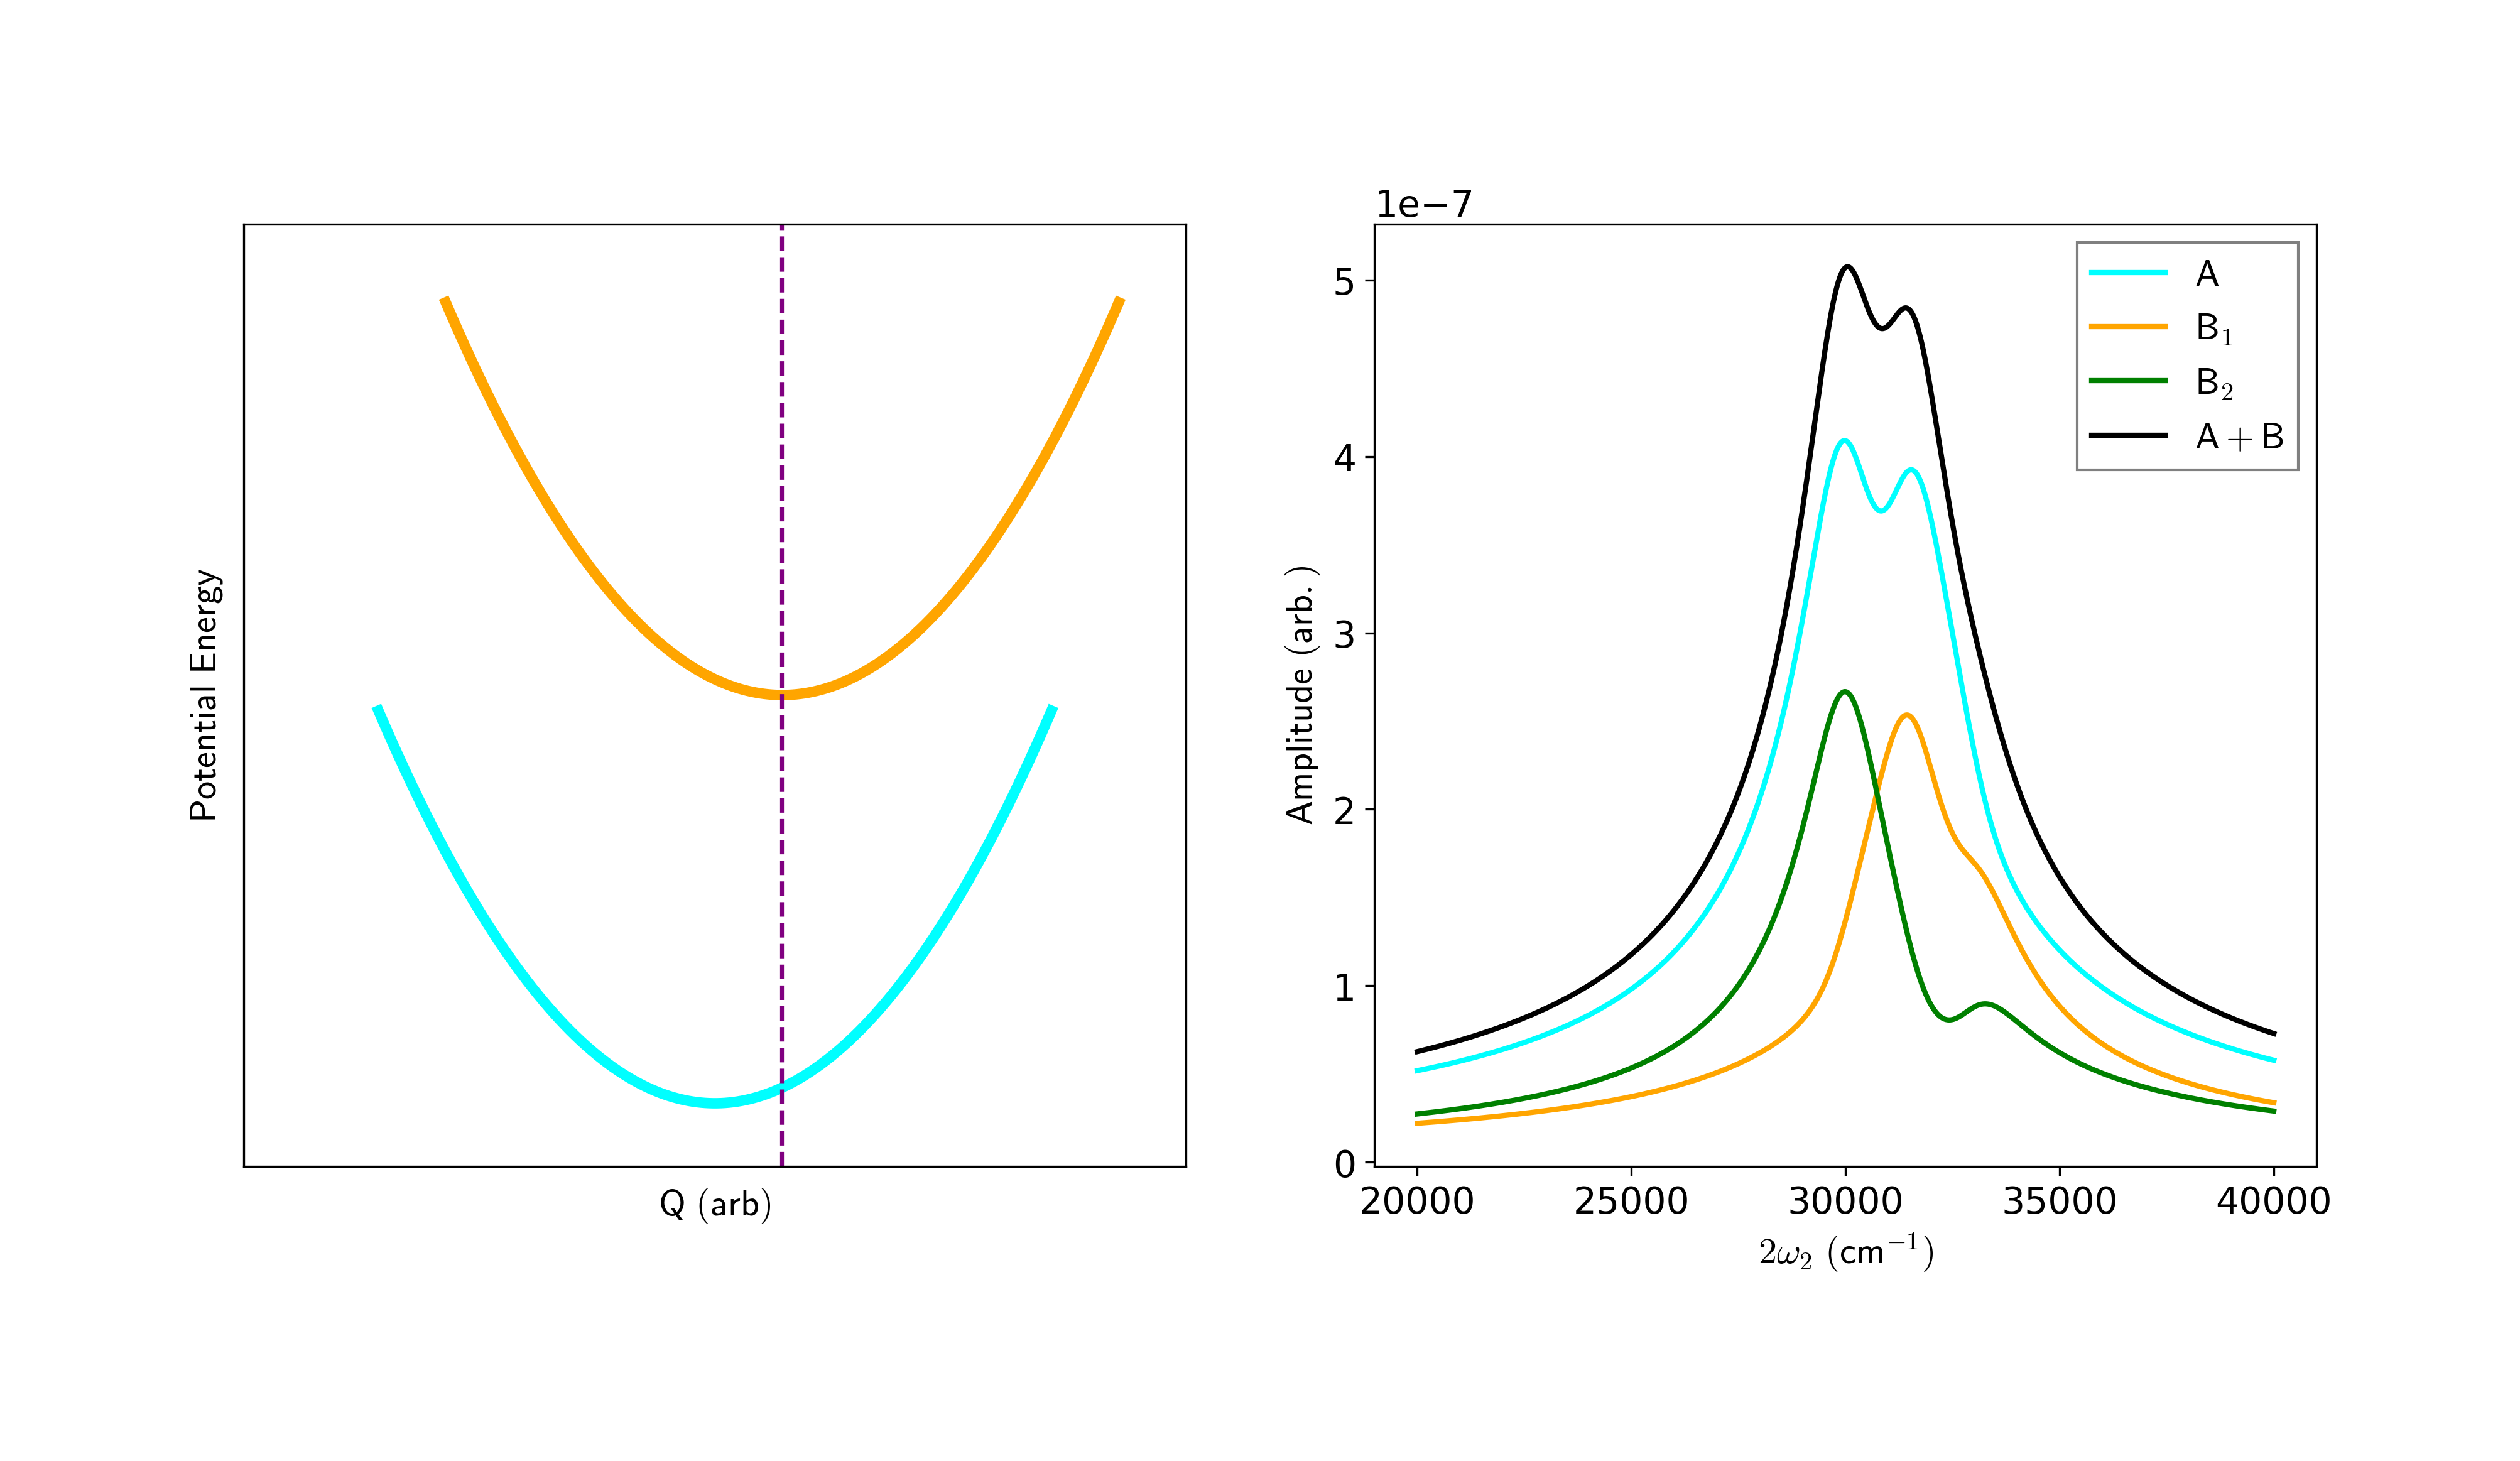
\includegraphics[width=6.66in]{drsive_spectrum.png}
	\caption{Contributions of $A, B$ (\autoref{ABterms_DR}) to DR-HDFG spectrum for a simple two harmonic well system.
		(a) Potential energy surfaces for a two-well system, (b) 1D HDFG spectrum for $\xi = 0.5$, $\omega_1 = \omega_{g1, g0}$. 
		It is assumed that $\omega_2 = \omega_3$.
		Note that (b) shows magnitudes of the labeled quantities.
		The vibrational states on the $|g)$ and $|e)$ manifolds are spaced 2200 cm$^{-1}$ apart, with the vibronic states $\ket{e,v'}$ given linewidths of 700 cm$^{-1}$ and $\hbar \omega_{eg}$ = 30000 cm$^{-1}$.
		Dotted lines in (b) denote the $v'$ = 0, 1, 2 vibronic resonances. 
		The vibronic one and two photon absorption operators are scaled such that $\abs{B_j}/\abs{A} \sim$ 0.01}
	\label{fig:doubres_spec}
\end{figure*}

The impact of vibronic coupling in the 2D spectrum is made clear by using a simple model. \cite{Kundu2022}
Using a two-well system described by 
\begin{subequations}
	\begin{equation}
		H_g = \frac{p^2}{2m} + \frac{1}{2} \hbar \omega q^2
	\end{equation}
and
	\begin{equation}
		H_e = \frac{p^2}{2m} + \frac{1}{2} \hbar \omega (q-\xi)^2 +\hbar \omega_{eg}
	\end{equation}
\end{subequations}
for the ground ($H_g$) and first excited ($H_e$) states, where $p$ is the momentum of the normal mode, the A and B contributions can be evaluated using Franck-Condon and Herzberg-Teller integrals tabulated in terms of the dimensionless normal mode $q$ and offset parameter $\xi$ (\autoref{fig:doubres_spec}a). \cite{Carlson1988thesis} 
Note that $q = m \sqrt{\omega/\hbar} Q$.
The spectrum is simulated for an electronic state which is both one and two photon allowed.
A simulated spectrum   (\autoref{fig:doubres_spec}b) highlighting the contributions of these terms on potential wells with $\xi = 0.5$ dissects the $A$ and $B$ contributions to the DR-SIVE spectrum.
Note that unlike resonant hyper-Raman spectra, which allow transitions between different normal modes, the use of the infrared pulse provides a type of site selectivity,\cite{RN103} so that only the normal mode which $\omega_1$ pumps can be involved in the vibronic coupling analysis.
This stimulated hyper-Raman type spectrum would be the expected result in a DR-HDFG experiment when investigating the vibronic structure of the electronic state coupled to $\ket{g,v}$.

Simulating the DR-HDFG spectrum for the simple two-well system allows dissection of selection rules and spectral signatures without the need for complex couplings.
There are two relevant regions of interest: the resonant region (2$\omega_2$ $\in$ [29000, 35000] cm$^{-1}$) and the non-resonant region.
Focusing far away from the resonant region ($2\omega_2 \sim$ 20000 cm$^{-1}$), it is clear that $A$ term response is non-negligible. 
As discussed above, the $A$ term in singly resonant HDFG vanishes when truly non-resonant.
However, the simulated spectrum shows a non-negligible $A$ term contribution to DR-HDFG output well beyond $\sim$ 20000 cm$^{-1}$, the limit for this model system where $\abs{\omega_{ev',g0} - 2\omega_2} \gg 2\Gamma_{ev',g0}$.
As such, it may be difficult to truly eliminate $A$ term resonances in HDFG spectra, even when largely detuned ($>$ 10000 cm$^{-1}$) from the electronic state. 

In the resonant region, the $A$ term contains character from all three possible transitions between $\ket{g,0}$, $\ket{e,v'}$ and $\ket{g,1}$. 
Significant contributions from $\ket{e,0}$ and $\ket{e,1}$ in the spectrum correspond well with expectations given the relative wavefunction overlap in \autoref{fig:doubres_spec}a. 
The small contribution to $A$ involving transitions with $\ket{e,2}$ is consistent with the large change in quantum number from $\ket{g,0}$ and its considerable displacement from the equilibrium point of $|g)$.
The dependence of $A$ on these Franck-Condon factors is in agreement with expectations following \autoref{ABterms_DR}. 

Unlike $A$ term contributions, the $B_1$ and $B_2$ terms are dependent upon both Franck-Condon and Herzberg-Teller contributions.
Based upon the disparity in transition amplitudes in the $B_1$ and $B_2$ terms for each vibronic transition, it is clear that the $B$ terms are sensitive to the Herzberg-Teller coupling integrals.
The $B_1$ term, whose vibronic coupling term is involved in the two-photon absorption event from $|g)$ to $|e)$, seemingly has minimal $0-0$ contributions. 
This is expected, as the Herzberg-Teller integral $\mel{0}{Q}{0}$ is smaller than $\mel{1}{Q}{0}$ and $\mel{2}{Q}{0}$. 
An explanation for the contribution from the $0-1$ transition in $B_2$ is similar.
Vibronic contributions to $B_2$ arise from the one photon emission transition; $\mel{1}{Q}{1}$ is smaller than the $\mel{1}{Q}{0}$ and $\mel{1}{Q}{2}$ contributions to the $B_2$ term.
However, the $0-2$ transition is smaller in amplitude than the $0-1$ transition because it is also dependent upon a $\langle 2 | 0 \rangle$ Franck-Condon factor.
In a realistic molecular system, where higher order contributions (e.g. Duschinsky coupling) effect vibronic coupling signatures, the spectral signatures will change to incorporate anharmonicites. \cite{Duschinsky1937, Carlson1990, Kundu2022}
However, investigating coupling between $\ket{g,2v}$ and the same $\ket{e,v'}$ vibronic states will likely assist in dissecting the site-selective electronic spectra.

\section{Quantitative Aspects of HDFG}\label{quant}
HDFG is dependent upon a hyper-Raman transition, which is several orders of magnitude weaker than Raman transitions.\cite{RN515}
As a result, it is useful to identify how HDFG output compares to a corresponding Raman based nonlinear spectroscopy.
Since the hyper-Raman process is stimulated by a two-photon process, a setup using only one optical parametric amplifier can perform a coherent four wave mixing hyper-Raman experiment by investigating $-\vec{k}_1 + 2\vec{k}_2$ processes (i.e. two laser CMDS), assuming a two photon absorption from a single pulse stimulates the hyper-Raman process.
A commonly used two laser CMDS method is vibrational sum frequency generation (vSFG), a $\chi^{(2)}$ technique whose phasematching is dictated by $\vec{k}_1 + \vec{k}_2$.
SFG output scales as $\chi^{(2)}_{IJK} \sim \langle \alpha_{ij} \mu_k \rangle$, where $\alpha_{ij}$ is the Raman polarizability tensor.
Both processes can be phasematched in media with normal indices of refraction, unlike the $\vec{k}_1 + 2\vec{k}_2$ HSFG process (\autoref{fig:comparisonwmel}).\cite{RN120}
Macroscopically, oddness in spatial inversion of the vSFG polarization eliminates output from centrosymmetric species under the electric dipole approximation.\cite{RN132, RN133}
As a result, the output of vSFG is significantly reduced relative to most third order spectroscopies because the output depends on surface number density, many orders of magnitude smaller than the bulk surface density. 
To motivate the application of HDFG spectroscopy, we perform a calculation to compare HDFG and vSFG output, where absorption effects are neglected for simplicity.

The output polarizations under the electric dipole approximation are written as
\begin{widetext}
	\begin{subequations}
	\begin{equation}
		\abs{P^{(2)}_{\text{vSFG}}} = \frac{N_{surf}}{\ell} F(\omega_1+\omega_2) \abs{\langle \alpha_{ij}\mu_{k} \rangle E(\omega_2)E(\omega_1)} 
	\end{equation}
	\begin{equation}
		\abs{P^{(3)}_{\text{HDFG}}} = N_{bulk}  F(2\omega_2-\omega_1) \abs{\langle \beta_{ijk} \mu_{l} \rangle E{(\omega_2)}E(\omega_2)E(-\omega_1)}
	\end{equation}
\end{subequations}
\end{widetext}
where N$_{bulk}$ is the bulk number density, and N$_{surf}$ is the surface number density ($\sim$ 10$^{16}$ m$^{-2}$ for H$_2$O adsorbed at quartz).\cite{RN133, Du1994}	
We assumed here that $\int_{0^-}^\ell \mathrm{d}z \langle \alpha_{ij}\mu_{k} \rangle \approx \ell \langle \alpha_{ij}\mu_{k} \rangle$, where $z$ is oriented along the surface normal and $0^{-}$ is the edge of the interface where substrate begins. \cite{RN133}
We take the film thickness ($\ell$) that can be probed by vSFG to be 1 nm, much less than the vSFG coherence length.\cite{RN133, Su1998}
For liquids with molar masses less than $\sim$100 g mol$^{-1}$ and densities roughly equal to that of H$_2$O$_{(l)}$ at room temperature, N$_{bulk} \sim$ 10$^{28}$ m$^{-3}$.
A normal dispersion curve is assumed so that $F(\omega_1+\omega_2) \approx F(2\omega_2-\omega_1)$.
To simplify analysis, orientational averaging is ignored (e.g., $\langle \beta_{ijk} \mu_{l} \rangle \approx \beta \mu$) and the input and output fields are taken to be co-polarized, so that
\begin{equation}
		P_{ratio} \equiv \frac{\abs{P^{(3)}_{\text{HDFG}}}}{\abs{P^{(2)}_{\text{vSFG}}}} \approx \frac{N_{bulk}}{N_{surf}} \frac{\beta}{\alpha} E(\omega_2) \ell \sim 10^3 \frac{\beta}{\alpha} E(\omega_2)\\
\end{equation}
Ziegler has noted that for a field with intensity 10 GW/cm$^{2}$, $\frac{\beta E}{\alpha} \sim 10^{-3} $ for vibrational modes when $E(\omega_2)$ is largely detuned from electronic resonances. \cite{RN515}
Such an intensity is easily obtained using modern ultrafast sources.
In this limit, $P_\text{ratio} \sim 1$.
Since the intensity ratio scales as $\abs{P_{ratio}}^2$, we see that the HDFG output is roughly as strong as vSFG, assuming only interfacial contributions in vSFG.
It is important to note that this calculation assumed negligible dipole and Raman polarizability dependence upon the distance from surface normal, ignored orientational averaging effects, and presumed equivalence of local field factors, all of which can significantly reduce output from either process. 
Nevertheless, since HDFG produces a number of photons similar to that of vSFG, HDFG is a viable technique for investigating bulk systems.

With the selection rules of HDFG understood for vibrational spectroscopy, and with HDFG generating a large enough output polarization, it becomes possible to extract quantitative information from its spectra.
Lineshape analysis is essential for extracting quantitative information from CMDS spectra.
Scanning across resonances create dispersive lineshapes, i.e, self-heterodyning, which inform on $\Re(\chi^{(3)})$ and $\Im(\chi^{(3)})$.\cite{Levenson1974_1, Levenson1974_2}
In the method introduced by Levenson and Bloembergen (Bloembergen Interferometry Experiment), an internal standard interferes with the resonant lineshape.
Self-heterodyning of the internal standard signal measures $\chi^{(3)}$ and does not require measurement of absolute intensities. 
Resonant lineshapes are also complicated by amplitude level interference between the sample,  substrate and/or sample cell windows, which must be accounted for to obtain quantitatively correct $\chi^{(3)}$ values. \cite{RN362, RN418}
Most quantitative methods in an n$^{th}$ order CMDS experiment are used to extract $\chi^{(n)}$ values to compare the relative strength of nonlinear processes in different media. \cite{Zhu87, RN351, RN345}
The recorded $\chi^{(n)}$ values provide insight into how microscopic quantities ($\vec{\mu}, \alpha_{ij}, \beta_{ijk}$) impact nonlinear output.
These quantities are usually extracted from their incoherent analogues (IR spectroscopy, spontaneous Raman spectroscopy, spontaneous hyper-Raman spectroscopy). \cite{Levenson1974_2, RN412, Shoute2005}

Calculating $\beta_{ijk}$ values from hyper-Raman experiments is difficult and has only been performed for a few molecular vibrations. \cite{Xu1997, Shoute2005, Kelley2010}
Methods reported in the literature to measure absolute hyper-Raman polarizabilities depend upon external standards such as hyperpolarizabilities of dissolved samples or two-photon absorption cross sections, also difficult to measure.
Since the Bloembergen interferometry experiment only relies on the third order susceptibility for measured species (e.g., benzene or CaF$_2$),\cite{Levenson1974_2} it is possible to use quantitative four wave mixing spectroscopy to calculate $\beta_{ijk}$ values.
It is thus useful to investigate how a treatment of orientational averaging can extract $\beta_{ijk}$ from the HDFG $\chi^{(3)}_{IJKL}$ expression.

In HDFG, 
\begin{equation}\label{chi3}
\begin{split}
		\chi^{(3)}_{IJKL} &= NF(\omega_4) \langle \gamma_{ijkl} \rangle = -\frac{NF}{4D \hbar \varepsilon_0 \Delta_{gv}} \langle \beta_{ijk} \mu_l \rangle \rho_{gg}\\
\end{split}
\end{equation}
\autoref{chi3} cannot be used as written to extract $\beta_{ijk}$, as $\beta_{ijk}$ is a Hermitian operator, but $\Delta_{gv} \in \mathbb{C}$. 
However, since the real and imaginary components of $\chi^{(3)}$ can be measured through the Bloembergen interferometry experiment, and $\beta_{ijk}$ is present in either term, we can choose to focus on the real or imaginary part of $\chi^{(3)}$.
When resonant, $\Re(\chi^{(3)})$ vanishes.
As such, assuming resonance conditions, we investigate $\Im(\chi^{(3)})$, giving, 
\begin{equation}
	\langle \beta_{ijk} \mu_{l} \rangle = -\frac{4D \hbar \varepsilon_0}{NF} \Gamma_{gv} \frac{1}{\rho_{gg}} \Im(\chi^{(3)}_{IJKL})
\end{equation}
The steps behind orientational averaging of $\gamma_{ijkl}$, a rank four tensor in the molecular frame, are detailed elsewhere.\cite{Andrews1977, McDonnell2024}
Briefly, a tensor in the molecular frame, A$_{ijkl}$, is transformed into an element of the same tensor in the laboratory frame, A$_{IJKL}$, through A$_{IJKL}$ = $\theta^{ijkl}_{IJKL} A_{ijkl} = \langle A_{ijkl} \rangle$, where summation over repeated indices is implied and $\theta$ is the transformation operator. \cite{McDonnell2024}
Orientational averaging shows specific polarization schemes isolate linear combinations of different $\beta_{ijk}$ terms. \cite{Bersohn1966, Willetts1992, Kauranen1996}
By using the expansions of $\beta_{ijk}$ and $\mu_{l}$ to $\order{Q_n}$ found earlier, we see
\begin{equation}\label{betasive}
	\langle \frac{\partial \beta_{ijk}}{\partial Q_n} {\frac{\partial \mu_l}{\partial Q_n}} \rangle = -\frac{8D \varepsilon_0}{NF}  \frac{\Gamma_{gv} \omega_{vg}}{\rho_{gg}} {\Im(\chi^{(3)}_{IJKL})}
\end{equation}
Since $\abs{\mu}$, and by extension $\abs{\partial \mu / \partial Q}$, values can be extracted from FT-IR spectra, HDFG can give quantitative information on the magnitude of $\beta_{ijk}$ for infrared active vibrations.
Additionally, by using two different input frequencies to stimulate the hyper-Raman transition, the asymmetric properties of $\beta_{ijk}$ can be examined and quantified. \cite{Christie1971, Denisov1986, Kozich2007}
To our knowledge, no experiment has been performed which quantifies deviations of the asymmetric and symmetric components of $\beta_{ijk}$. 
These quantitative aspects of HDFG could prove useful to examine how well computational methods calculate $\beta_{ijk}$ values and the strength of spontaneous hyper-Raman scattering with non-degenerate pulses.

\section{Mixed-Domain HDFG}\label{mixeddomain}
The properties of steady state HDFG (complete pulse overlap) are useful for understanding the selection rules that drive HDFG output, motivating time domain experiments.
Time domain HDFG could be a useful alternative technique for measuring single quantum coherence dephasing times.
Working under the rotating wave approximation and neglecting spatial components, the output polarization is written in the time domain as 
\begin{equation}
	\begin{split}
			\vec{P}(t) &= \int_0^\infty \mathrm{d}t_3 \int_0^\infty \mathrm{d}t_2 \int_0^\infty \mathrm{d}t_1 R^{(3)}(t_1, t_2, t_3)  \vdots \vec{E}_3(t-t_3) \\
			&\vec{E}_2(t-t_3-t_2 - \tau_{23}) \vec{E}_1(t-t_3-t_2-t_1 - \tau_{13}) 
	\end{split}
\end{equation}
where the electric fields are labeled according to their placement in the WMEL diagrams, $\tau_{ij} = \tau_i - \tau_j$ is the time delay between pulses $i$ and $j$, and R is the response function. \cite{RN287} 
Here, we will focus on the response function formalism for singly resonant HDFG, as the extension to doubly resonant HSFG, easily transferable to DR-HDFG, has been treated by Cho. \cite{Cho2001}
The response function for the HDFG pathway illustrated in \autoref{fig:hdfg}a, assuming $\omega_2$ and $\omega_3$ are temporally overlapped, not electronically resonant, and $\rho(-\infty) = 1$, in the limit of homogeneous broadening is \cite{Cho2001, Meyer2004, RN367}
\begin{equation}
	R^{(3)}(t_1) = \frac{i}{\hbar} \beta_{ijk}(t_1) \mu_l(0) \exp(-i\Delta_{gv}t_1) \theta(t_1) 
\end{equation}  
where $\theta$ is the Heaviside function.
The pure time-domain HDFG output reports on the dephasing characteristics of the $\ket{g}\bra{v}$ coherence. 
This method provides practitioners of sum frequency generation the ability to probe isotropic dephasing dynamics without many meaningful changes in their optical setup, and thus compare $\ket{g}\bra{v}$ dephasing in the bulk and at the interface.\cite{RN224}

Transient HDFG spectroscopy, or pump-HDFG-probe, similar to transient vSFG spectroscopy, can be implemented to learn about relaxation dynamics in isotropic systems. \cite{RN224, Bonn2024}
A useful attribute of the $\beta_{ijk}$ dependence in HDFG output is added polarization control. 
Similar to SFG experiments that probe different elements of the infrared transition dipole and Raman polarizability tensors, probing different elements of $\beta_{ijk}$ in HDFG can greatly assist in understanding ultrafast dynamics in isotropic systems, as suggested by Seliya et al. \cite{Shen90, RN224, Bonn2024}
Polarization control in IR-pump-HDFG-probe, analogous to ultrafast transient absorption spectroscopy for vibrational modes, would be an interesting venue to assess the sensitivity of HDFG to different hyper-Raman tensor elements. 

It is well known that nonlinear wave mixing processes which share the same time ordering and output frequency will interfere. \cite{RN342, RN135}
Understanding interfering pathways is useful because they can eliminate nonlinear output. 
While we have only isolated one specific HDFG process so far, there are at least fourteen different WMELs which can provide HDFG output in the driven limit. \cite{RN352}
If $\omega_2$ ($\omega_1$) becomes resonant (non-resonant), then other HDFG pathways appear (\autoref{fig:sivewmel2}).\cite{McDonnell2024} 
While the methods in \autoref{fig:sivewmel2} possess identical selection rules to \autoref{fig:hdfg}, the WMEL diagrams presented in \autoref{fig:sivewmel2} will interfere, as they share the same phasematching condition but have oppositely signed amplitudes.
\begin{figure}[!htbp]
	\centering
	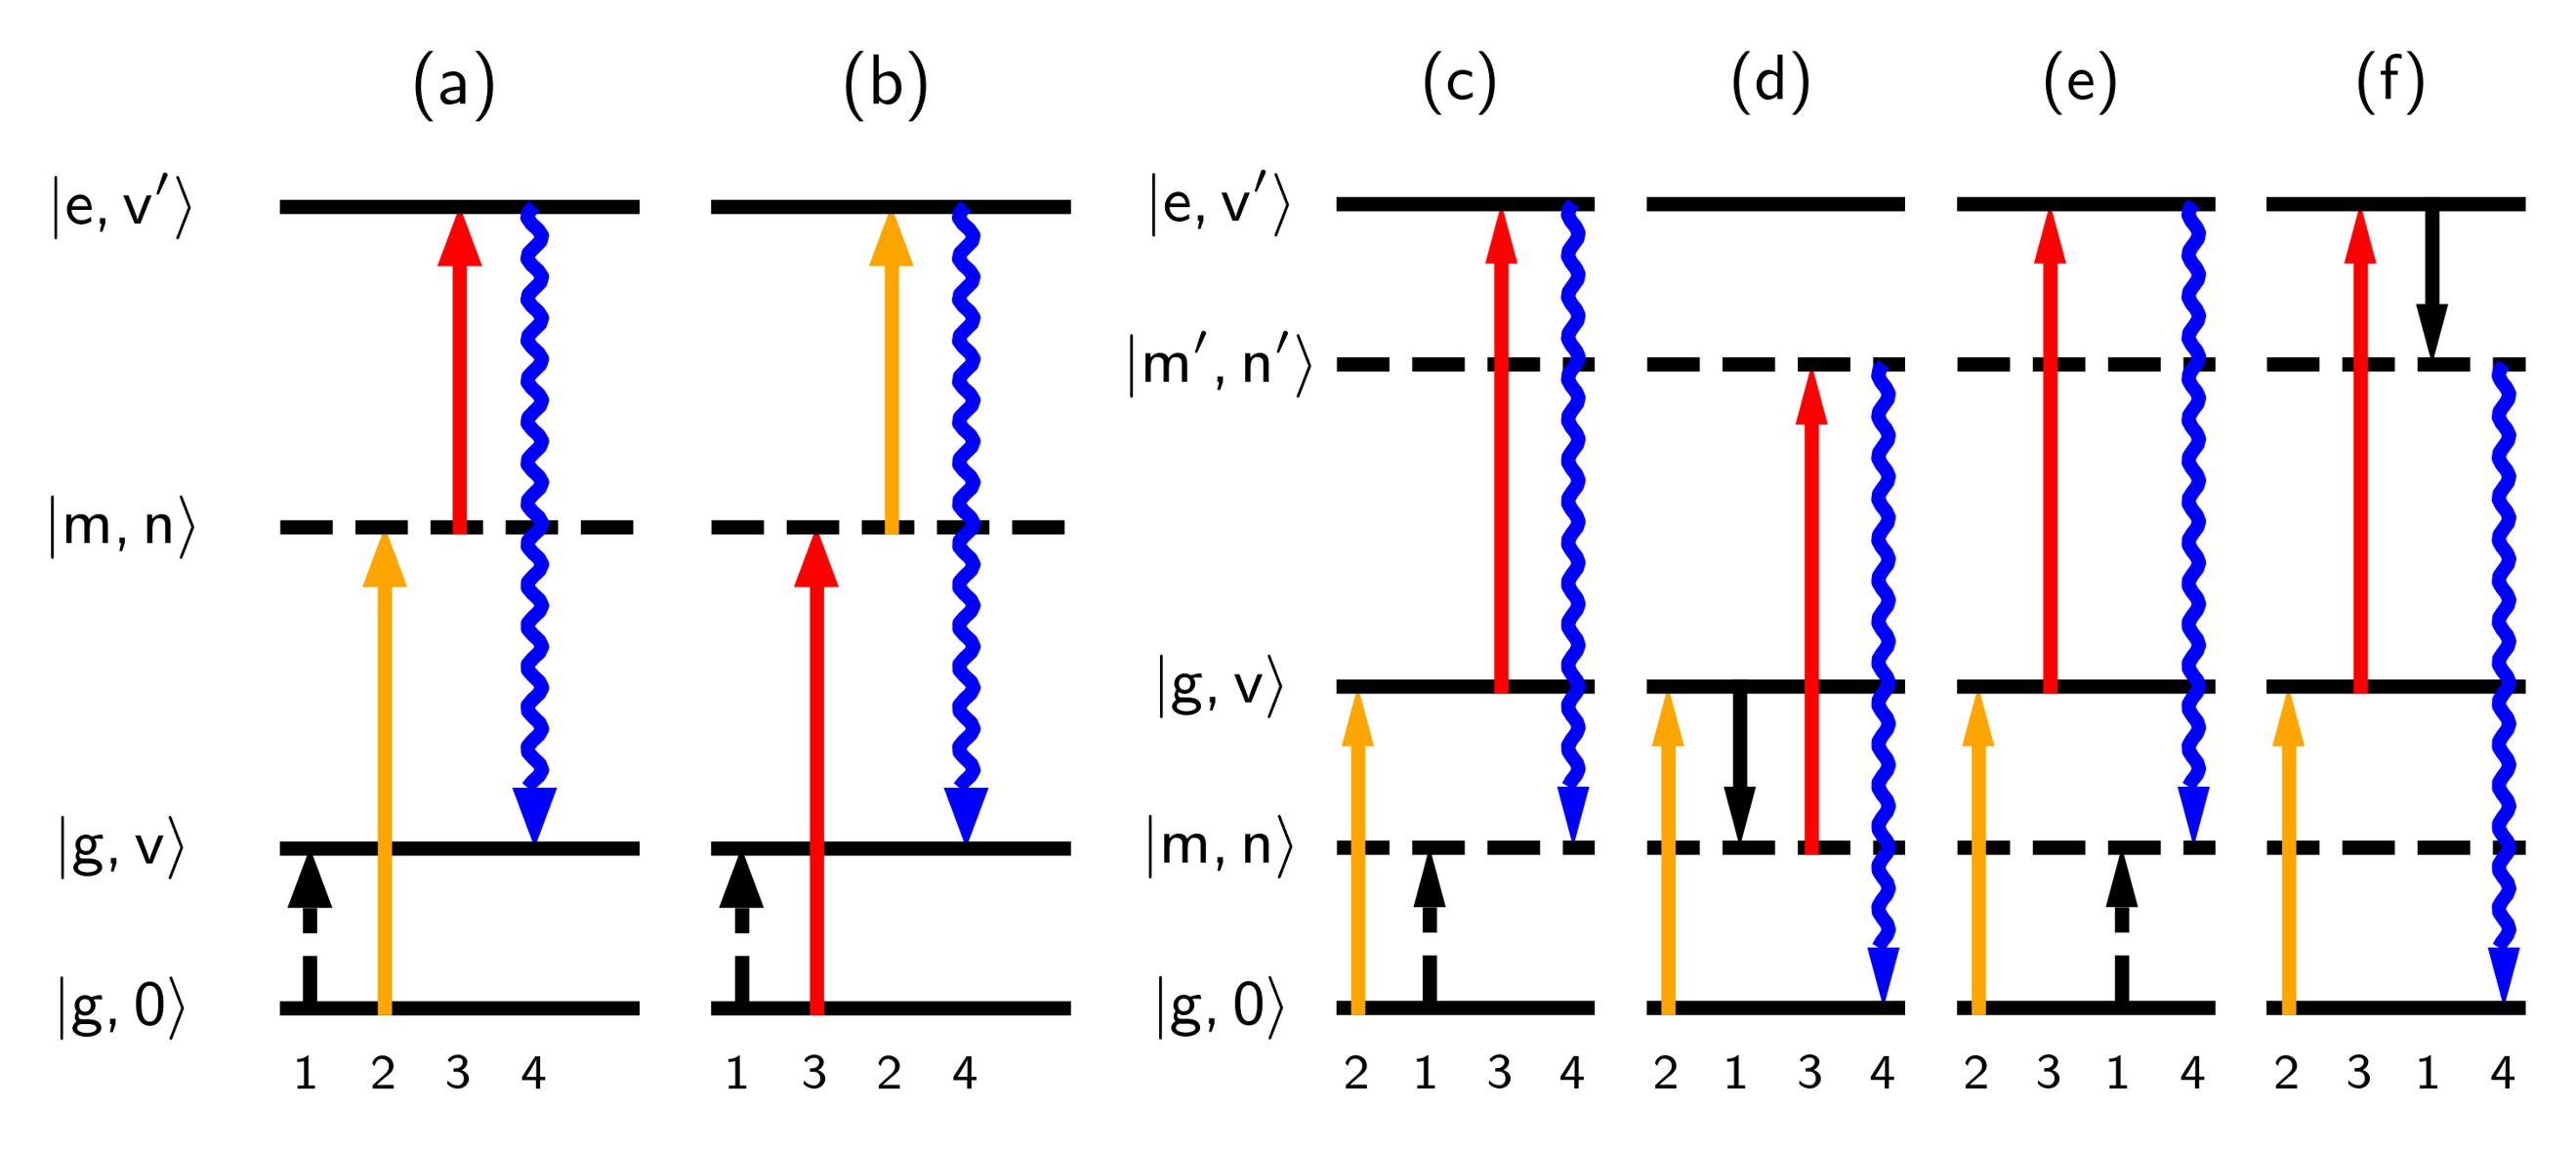
\includegraphics[width=3.375in]{figures/timeorderedwmel.png}
	\caption{WMEL diagrams of HDFG pathways in the  $\vec{k}_4 = -\vec{k}_1 + \vec{k}_2 + \vec{k}_3$ phasematching geometry when $\omega_2$ interacts with the system first. 
		}
	\label{fig:sivewmel2}
\end{figure}

The third order response functions for the pathways detailed in \autoref{fig:sivewmel2} when $\omega_1$ and $\omega_3$ are temporally overlapped, assuming $\rho(-\infty) = 1$, in the limit of homogeneous broadening are
\begin{subequations}
	\begin{equation} \label{mixing:a}
		R^{(3)}_{a} (t_2) = R^{(3)}_{c} (t_2) = -\frac{i}{\hbar} \beta_{ijk}(t_2) \mu_l(0)  \exp(-i\Delta_{vg}t_2) \theta(t_2)
	\end{equation}
	\begin{equation}\label{mixing:b}
			R^{(3)}_{b} (t_2) = R^{(3)}_{d} (t_2) = \frac{i}{\hbar} \beta_{ijk}(t_2) \mu_l(0)  \exp(-i\Delta_{vg}t_2) \theta(t_2)
	\end{equation}
\end{subequations}
The total response function in this time ordering is therefore $R^{(3)}_\text{tot} (t_2) = R^{(3)}_{a} (t_2) + R^{(3)}_{b} (t_2) + R^{(3)}_{c} (t_2) + R^{(3)}_{d} (t_2) = 0$. 
Since the total output response function vanishes in this time-ordering, the pathways in \autoref{fig:sivewmel2} perfectly destructively interfere.
Therefore, to measure dynamics via HDFG, the time ordering shown in \autoref{fig:hdfg} should be used.
These ideas have been seen experimentally in ultrafast DOVE work. \cite{RN367, McDonnell2024}
In the case of the \autoref{fig:hdfg}a time ordering, there are no opportunities for interference from other third order processes. 
However, a possible mechanism for interfering output in the \autoref{fig:hdfg}a pathway is a cascaded second order process (SFG, DFG). \cite{RN300}
While unimportant in achiral isotropic systems,\cite{Belkin2000} second order cascades may become important in media where SFG and DFG are allowed, e.g. chiral media, interfaces or noncentrosymmetric media. 

Combinations of time and frequency domain spectroscopy, also called mixed domain spectroscopy, are useful ways to understand frequency-dependent dynamics. \cite{RN135, RN367, RN171, RN131}
Mixed domain spectroscopy is a useful alternative to steady state spectroscopy as pulse separation can eliminate nonresonant background and isolate specific pulse ordering sequences. \cite{RN372, RN324, McDonnell2024}
Isolating different pulse orderings can isolate pathway specific signal and minimize interference from unwanted pathways which share the same phasematching constraints. 
Mixed domain HDFG can resolve frequency dependent free induction decay, which could prove useful for understanding isotropic dynamics of single quantum coherences. 
Mixed domain resonant HDFG, using pathways similar to those in \autoref{fig:hdfg}b, could also measure time-dependent electronic-vibrational fluctuations, as discussed by Cho. \cite{Cho2001}
These methods should be able to provide complimentary information to that found in 2D Electronic-Vibrational (2D-EV) spectroscopy. \cite{Dong2015, Lewis2015, Gaynor2017}

\section{Conclusions}
Coherent vibrational, hyper-Raman coherent four wave mixing spectroscopies are identified and discussed.
Singly resonant hyper difference frequency generation (SR-HDFG) processes are shown to be the coherent hyper-Raman analogue of infrared active vibrations.
We find that HDFG is always allowed for harmonic transitions, making it a potential tool for measuring single quantum coherence lifetimes. 
Through an examination of the hyper-Raman $A,B,C$ terms as they appear in the doubly resonant HDFG (DR-HDFG) output, the impact of vibronic coupling in DR-HDFG spectrum was examined.
It is found that the $A$ term dominates in DR-HDFG, but vanishes in SR-HDFG and select cases (e.g. centrosymmetry) in DR-HDFG. 
The non-Condon effects that are present in the absence of $A$ might prove useful for dissecting the structure of modes which involve particular IR active vibrations in vibronic coupling.
Through a simple treatment, it is seen that HDFG and vibrational sum frequency generation (vSFG) have roughly the same output intensities. 
This makes HDFG a reasonable spectroscopy for systems outside of the ideal solvents tested in the literature, and should be readily extended to a variety of non-ideal molecular and materials systems. 
Based upon a simple treatment of orientational averaging, we show that HDFG can extract the hyper-Raman hyperpolarizability without a need for technically difficult, analytically rigorous hyper-Raman scattering experiments. 
The HDFG method shows promise as a spectroscopic probe of unique electronic structure effects in a variety of molecular systems, but also for understanding the dynamics of single quantum coherences. 
\section{Data Availability}
The workup scripts which support this work can be found at [insert github link here].

\section{Acknowledgments}
This work received support from the Department of Energy, Office of Basic Energy Sciences, Division of Materials Sciences and Engineering (Grant no. DE-SC0002162).
R.P.M. acknowledges support from the NSF Graduate Research Fellowship Program (Grant no. DGE-2137424). 

%todo: figure out how footnotes work...

%{By defining $\Lambda^{mn}_{ij} = \sum_k (m|M_i|k) (k|M_j|n)$, expanding $\Lambda^{mn}_{ij}$ to $\order{Q}$ gives $\Lambda^{mn}_{0,ij} + \partial/ \partial Q \sum_k (m|M_i|k) (k|M_j|n) Q$ = $\Lambda^{mn}_{0,ij} + \sum_k (m|\partial M_i / \partial Q|k) (k|M_j|n) Q + (m|M_i|k) (k|\partial M_j / \partial Q|n) Q$, in agreement with the substitution made above.} 

\section{References}
% Create the reference section using BibTeX:
\bibliography{library.bib}

\end{document}
%


